
%\begin{figure}
	\centering
	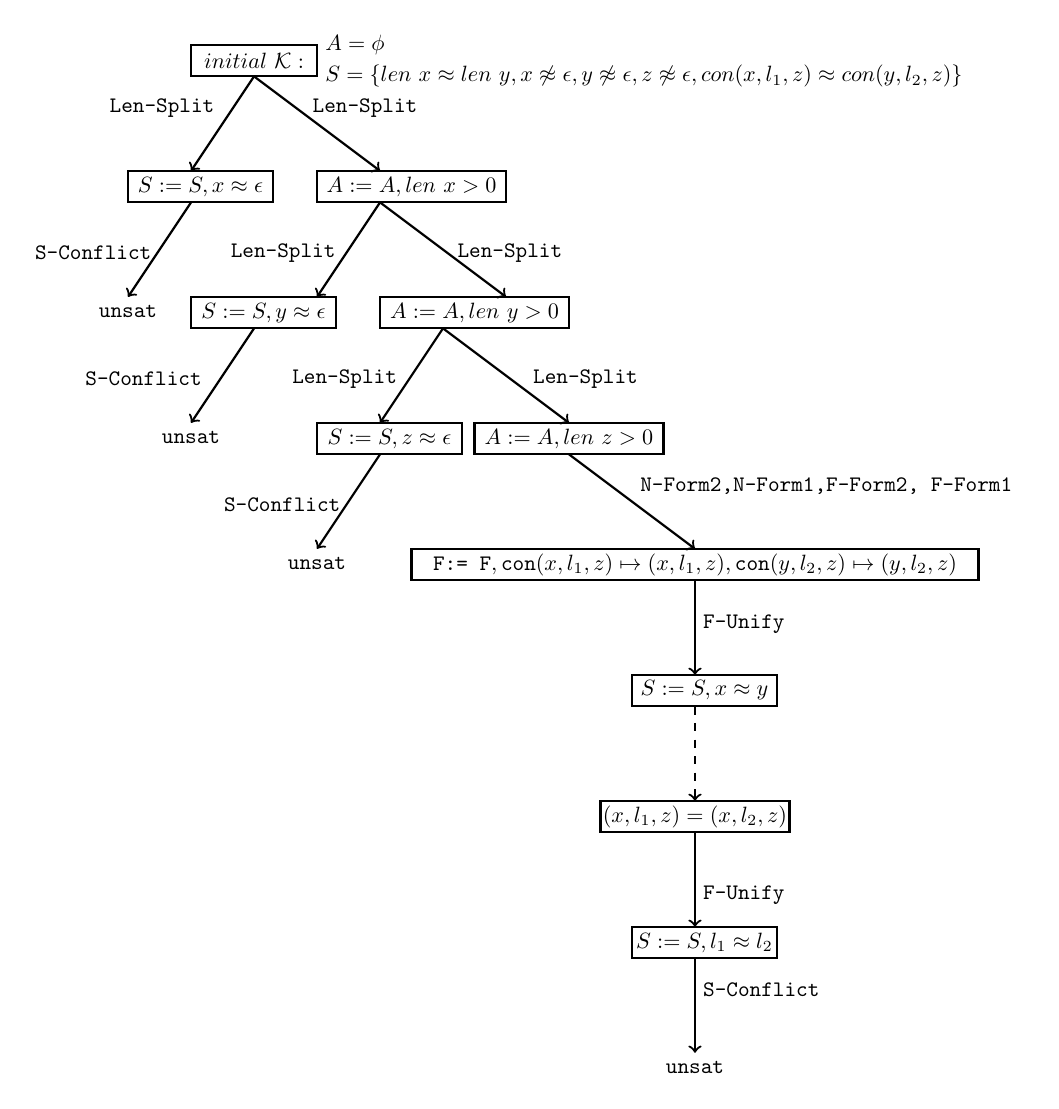
\begin{tikzpicture}[thick,scale=0.8, every node/.style={transform shape}]
	
	\node [right] at (3,20) { $ A=\phi $};
	\node [right] at (3,19.5) { $ S=\{  len \ x \approx len \ y, x \not\approx \epsilon, y \not\approx \epsilon,
		z \not\approx \epsilon, con (x, l_1,z) \approx con (y, l_2, z)\} $}; 
	 
    \draw (1,20) rectangle (3,19.5) node[pos=.5] {$ initial \ \mathcal{K}:$};
	
	\draw [->] (2,19.5) -- (1,18);
	\node [left] at (1.5,19) {$\texttt{Len-Split}$};
	
	\draw [->] (2,19.5) -- (4,18);
	\node [right] at (2.8,19) {$\texttt{Len-Split}$};
	
	
	\draw (0,18) rectangle (2.3,17.5) node[pos=.5] {$S:=S, x\approx \epsilon$};
	\node [rectangle, below] at (1,18) {};
	
	
	\draw (3,18) rectangle (6,17.5) node[pos=.5] {$A:=A, len \ x  > 0$};
	\node [rectangle, below] at (4,18) {};
	
	\draw [->] (1,17.5) -- (0,16);
	\node [left] at (0.5,16.7) {$\texttt{S-Conflict}$};
	
	\draw [->] (4,17.5) -- (3,16);
	\node [right] at (1.5,16.7) {$\texttt{Len-Split}$};
	\draw [->] (4,17.5) -- (6,16);
	\node [right] at (5.1,16.7) {$\texttt{Len-Split}$};
	
	\node [below] at (0,16) {$\texttt{unsat}$};
	\draw (1,16) rectangle (3.3,15.5) node[pos=.5] {$S:=S, y\approx \epsilon$};
	\node [below] at (2,16) {};
	\draw (4,16) rectangle (7,15.5) node[pos=.5] {$A:=A, len \ y  > 0$};
	\node [below] at (5,16) {};
	
	\draw [->] (2,15.5) -- (1,14);
	\node [left] at (1.3,14.7) {$\texttt{S-Conflict}$};
	\draw [->] (5,15.5) -- (4,14);
	\node [left] at (4.4,14.7) {$\texttt{Len-Split}$};	
	\draw [->] (5,15.5) -- (7,14);
	\node [right] at (6.3,14.7) {$\texttt{Len-Split}$};
	
	
	\node [below] at (1,14) {$\texttt{unsat}$};
	\draw (3,14) rectangle (5.3,13.5) node[pos=.5] {$S:=S, z\approx \epsilon$};
	\node [below] at (4,14) {};
	\draw (5.5,14) rectangle (8.5,13.5) node[pos=.5] {$A:=A, len \ z  > 0$};
	\node [below] at (7,14) {};


	\draw [->] (4,13.5) -- (3,12);
	\node [left] at (3.5,12.7) {$\texttt{S-Conflict}$};
	\draw [->] (7,13.5) -- (9,12);
    \node [right] at (8,13) {$\texttt{N-Form2,N-Form1,F-Form2, F-Form1 }$};
    

	
	\node [below] at (3,12) {$\texttt{unsat}$};
	\draw (4.5,12) rectangle (13.5,11.5) node[pos=.5] {$\texttt{F:= F},\texttt{con}(x,l_1,z)\mapsto (x,l_1,z),\texttt{con}(y,l_2,z)\mapsto(y,l_2,z)$};
	\node [below] at (9,12) {};
	
	\draw [->] (9,11.5) -- (9,10);
	\node [right] at (9,10.8) {$\texttt{F-Unify}$};
	
	\draw (8,10) rectangle (10.3,9.5) node[pos=.5] {$S:=S, x\approx y$};
	\node [below] at (9,10) {};
	
	\draw [dashed,->] (9,9.5) -- (9,8);
	
	\draw (7.5,8) rectangle (10.5,7.5) node[pos=.5] {$( x, l_1, z ) = (x, l_2,z)$};
	\node [below] at (9,8) {};
	
	\draw [->] (9,7.5) -- (9,6);
	\node [right] at (9,6.5) {$\texttt{F-Unify}$};
	
	\draw (8,6) rectangle (10.3,5.5) node[pos=.5] {$S:=S, l_1 \approx l_2$};
	\node [below] at (9,6) {};
	
	\draw [->] (9,5.5) -- (9,4);
	\node [right] at (9,5) {$\texttt{S-Conflict}$};
	
	\node [below] at (9,4) {$\texttt{unsat}$};
	
	
	
	
	
	
	\end{tikzpicture}
	\caption{The derivation tree for example 1. Here $l_1, l_2 $ are distinct constants of same length.}
\end{figure}	





\begin{figure}[ht]
	\centering
 	\begin{minipage}[t]{0.45\linewidth}
 		\begin{tikzpicture}[->,>=stealth',
 		shorten >=1pt,auto,node distance=0.5cm,thick,
 		main node/.style={rectangle,draw}, text node/.style={rectangle}]
 		
 		
 		\node  (s1){$s_1: x =  \texttt{con}("ab", z) $};
 		\node  (s2) [below of=s1] {$s_2: y =  \texttt{con}("de", z) $};
 		\node  (s3) [below of=s2] {$s_3: y =  \texttt{con}("abc", l)$};
 		\node  (s4) [below of=s3] {$s_4: x =  y$};
 		\node  (s5) [below of=s4] { $s_5: \texttt{len}\  x > 6$};
 		\node  (s6) [below of=s5] {$assert( s_1 \wedge (s_2 \vee s_3 ) \wedge s_4 \wedge s_5)$};
 		
 		
 		\end{tikzpicture}
 	\end{minipage}
	\quad
	\centering
	\begin{minipage}[t]{0.45\linewidth}
		\begin{tikzpicture}[->,>=stealth',
		shorten >=1pt,auto,node distance=2.3cm,thick,
		main node/.style={rectangle,draw}, text node/.style={rectangle}]
		
		\node (root) {$ s_1 \wedge (s_2 \vee s_3 ) \wedge s_4 \wedge s_5$};
		\node[main node] (sat-solver) [below of=root] {SAT-Solver};
		\node[main node] (t-solver-1) [below left of=sat-solver] {$\mathcal{T}$-Solver};
		\node[main node] (t-solver-2) [below right of=sat-solver] {$\mathcal{T}$-Solver};	
		\node[text node] (sat) [below of=t-solver-2] {$ \texttt{sat}$};
		
		
		\path[every node/.style={font=\sffamily\small}]
		(root) edge node [left] {} (sat-solver)	
		
		(sat-solver) edge node [right, near end] { $s_1 ,s_2 ,  s_4, s_5$} (t-solver-1)
		(sat-solver) edge node [right] {$s_1 ,s_3 ,  s_4, s_5$} (t-solver-2)	
		(t-solver-1) edge [bend left] node [left] {unsat} (sat-solver)	
		(t-solver-2) edge  node [right] {} (sat);
		\end{tikzpicture}
	\end{minipage}
	\caption{On the left the set of constraints and the boolean formula. And on the right side the interaction with SAT-Solver core and theory solver is shown.}
	\label{smt_example_1_2}
\end{figure}

	\begin{figure}
		\centering	
		\begin{tikzpicture}[->,>=stealth',
		shorten >=1pt,auto,node distance=2cm,thin,
		main node/.style={rectangle,draw}, text node/.style={rectangle}]
		
		
		\node [left] at (-10mm,0) {$ \{s_1, s_2, s_4,  s_5\}$};
		\node[main node] (a) {$initial\ \mathcal{K}$};
		\node[main node] (b) [below left of=a] {$S:=S, x\approx \epsilon$};
		\node[main node] (c) [below right of=a] {$A:=A, len\ x > 0$};
		
		\node[main node] (d) [below left of=b] {$unsat$};
		\node[main node] (e) [below left of=c] {$S:=S, y\approx \epsilon$};
		\node[main node] (f) [below right of=c] {$A:=A, len\ y > 0$};
		
		\node[main node] (g) [below left of=e] {$unsat$};
		\node[main node] (h) [below left of=f] {$S:=S, z\approx \epsilon$};
		\node[main node] (i) [below right of=f] {$A:=A, len\ z > 0$};
		
		\node[main node] (j) [below left of=h] {$unsat$};
		\node[main node] (k) [below of=i] {$\{ x,y,con(ab,z),con(de,z)\}$};
		
		\node [draw] (l) at (43mm,-75mm)  {$unsat$};
		
		
		\path[every node/.style={font=\sffamily\small}]
		(a) edge node [left] {\texttt{Len-Split}} (b)
		(a) edge node [right] {\texttt{Len-Split}} (c)
		(b) edge node [left] {\texttt{S-Conflict}} (d)
		(c) edge node [left] {\texttt{Len-Split}} (e)
		(e) edge node [left] {\texttt{S-Conflict}} (g)
		(c) edge node [right] {\texttt{Len-Split}} (f)
		(f) edge node [left] {\texttt{Len-Split}} (h)
		(f) edge node [right] {\texttt{Len-Split}} (i)
		(h) edge node [left] {\texttt{S-Conflict}} (j)
		(i) edge node [left] {normalization} (k)
		(k) edge node [left] {\texttt{S-Conflict}} (l);
		
		\end{tikzpicture}			
		\caption{The branch of derivation tree, which ends up in \texttt{unsat}.}
		\label{leftDerivationTree}
	\end{figure}
	\begin{figure} 	
		\centering
		\begin{tikzpicture}[->,>=stealth',
		shorten >=1pt,auto,node distance=1.3cm,thin,
		main node/.style={rectangle,draw}, text node/.style={rectangle}]
		
		
		\node [left] at (-10mm,0) {$ \{s_1, s_3, s_4,  s_5\}$};
		\node[main node] (a) {$initial\ \mathcal{K}$};
		\node (dummy) [below of=a] {};
		%\node[main node] (b) [left of=dummy] {$unsat$};		
		\node [draw] (b) at (-25mm,-12mm)  {$unsat$};
		\node[main node] (c) [right of=dummy] {$\{ x,y,con(ab,z),con(abc,l)\}$};
		\node[main node] (d) [below of=c] {$S:=S, z \approx con(c, l)$};
		\node[main node] (e) [below of=d] {$A:=A, len\ z \approx 1 + len l$}; 
		\node[main node] (f) [below of=e] {$A:=A, len\ l > 3$};
		\node[main node] (g) [below of=f] {$saturation$};
		
		\node at (7mm,-72mm) {$ l \approx "AAAA" \mapsto z \approx "cAAAA" \mapsto x, y\approx "abcAAAA"$};
		
		\path[every node/.style={font=\sffamily\small}]
		(a) edge [dashed] node [left] {\texttt{Len-Split}} (b)
		(a) edge [dashed] node [right] {\texttt{Len-Split}} (c)
		(c) edge  node [right] {\texttt{F-Unify}} (d)
		(d) edge [dashed] node [right] {\texttt{Len}} (e)
		(e) edge  node [right] {normalization} (f)
		(f) edge  node [right] {normalization} (g);
		
		
		\end{tikzpicture}			
		\caption{The branch of derivation tree, which ends up in saturation.}
		\label{rightDerivationTree}
	\end{figure}		
	
	
